\documentclass[11pt, twoside]{memoir}

\setsecnumdepth{subsubsection}
\settocdepth{subsubsection}

\usepackage[normalem]{ulem}

\usepackage{fontspec}
	\setmainfont%
		[Mapping=tex-text]
	{Cambria}
	\setsansfont%
%	[Ligatures={NoCommon, NoDiscretionary},%
		[Mapping=tex-text]%
		{Inconsolata}
\usepackage{relsize}

\def\textlabel#1{{\relsize{-.5}\fontspec[Mapping=tex-text]{Roboto Mono}{#1}}}
\def\langtext#1{\textit{#1}}

\usepackage{float}

\usepackage[top=1in, bottom=1in, left=1.25in, right=1.25in]{geometry}

\usepackage{xcolor}

\usepackage{hyperref}

\renewcommand\cftappendixname{\appendixname~}
\usepackage[nonumberlist, nopostdot, section=chapter, numberedsection=autolabel]{glossaries}
\makeglossaries

\usepackage{tikz}
\usetikzlibrary{shapes, arrows, backgrounds, fit, positioning}
\usetikzlibrary{decorations.pathreplacing}
\tikzset{
    dots/.style={
        line width=4pt,
        line cap=round,
        dash pattern=on 0pt off 6pt
    }
}
\usepackage{colortbl}
	\definecolor{CB1}{RGB}{0, 114, 178}%BLUE
	\definecolor{CB2}{RGB}{213, 94, 0}%VERMILLION
	\definecolor{CB3}{RGB}{0, 158, 115}%BLUE GREEN
	\definecolor{CB4}{RGB}{204, 121, 167}%REDDISH PURPLE
	\definecolor{CB5}{RGB}{86, 180, 233}%SKY BLUE
	\definecolor{CB6}{RGB}{230, 159, 0}%ORANGE
	\definecolor{CB7}{RGB}{240, 228, 66}%YELLOW
	\def\CB#1#2{\textcolor{CB#1}{#2}}
\usepackage{booktabs, longtable, array, arydshln, multirow}
\usepackage{caption}
\newlength\defaultaboverulesep
\setlength\defaultaboverulesep{\aboverulesep}
\newlength\defaultbelowrulesep
\setlength\defaultbelowrulesep{\belowrulesep}
\setlength\aboverulesep{0pt}
\setlength\belowrulesep{0pt}
\def\arraystretch{1.15}

\usepackage[framemethod=tikz]{mdframed}
	\newmdenv[middlelinecolor=CB1,
		middlelinewidth=1pt,
		backgroundcolor=gray!50,
		roundcorner=4pt]{infobox}
	\newmdenv[middlelinecolor=CB2,
		middlelinewidth=2pt,
		backgroundcolor=CB2!30,
		roundcorner=4pt]{toexpand}

\usepackage{makeidx}
\usepackage{graphicx}
	\graphicspath{{figures}}

\usepackage{expex}

\usepackage{enumitem}
	\setitemize{itemsep=.5ex, topsep=1ex, parsep=0pt, partopsep=0pt, leftmargin=3em, rightmargin=0ex}
	\setenumerate{itemsep=.5ex, topsep=1ex, parsep=0pt, partopsep=0pt, leftmargin=3em, rightmargin=0em}
\usepackage[hang, flushmargin, multiple, bottom, stable]{footmisc}

\usepackage{fancyhdr}

\usepackage{natbib}
	\bibpunct[:]{(}{)}{,}{a}{}{,}
	\setlength{\bibsep}{1ex plus 0.3ex}
\renewcommand{\bibsection}{\part*{Bibliography}}

\usepackage{cite-ref-errors}

\setlength\parskip{.5\baselineskip}
\setlength\parindent{0pt}
\frenchspacing
\raggedbottom

\def\THIStitle{Embarking on PoLaR Explorations}
\def\THISsubtitle{A Framework for Intonational Annotation and Analysis}
\pagestyle{fancy}
	\fancyhead[LO]{\textit{\THIStitle}}
	\fancyhead[RO]{}
	\fancyhead[LE]{}
	\fancyhead[RE]{Ahn, Veilleux, Shattuck-Hufnagel, Brugos}
\pagestyle{plain}
\hypersetup{
	breaklinks=true,
	pdfauthor={Byron Ahn, Nanette Veilleux, Stefanie Shattuck-Hufnagel, and Alejna Brugos},
	pdftitle={\THIStitle: \THISsubtitle},
	bookmarks,
	bookmarksopen=true,
	colorlinks=false,
	allcolors=blue
}

\makeindex

\begin{document}
\frontmatter
\captionsetup{margin=1.5cm, skip=4pt, labelfont={bf, footnotesize}, textfont={footnotesize}}

\title{\THIStitle}
\author{Byron Ahn \and Nanette Veilleux \and Stefanie Shattuck-Hufnagel \and Alejna Brugos}
\date{\today}
%{\normalsize\textcolor{red}{These guidelines are still under active development.\\Find the latest version of the guidelines, as well as .wav files, .TextGrid files, and some scripts, at \url{https://www.polarlabels.com/}.}}

\begin{titlingpage}
\vspace*{\fill}
\begin{center}
\textbf{\huge{\THIStitle:\strut}}\\
\textbf{\huge{\THISsubtitle\strut}}
\\[6\baselineskip]
{\large{Byron Ahn,\strut\\Nanette Veilleux,\strut\\Stefanie Shattuck-Hufnagel,\strut\\and Alejna Brugos\strut}}\\[6\baselineskip]
{\large\textit{draft}}\\
November 2022
\end{center}
\vspace*{\fill}
\end{titlingpage}

\tableofcontents
\newpage
\listoffigures
\listoftables
\newpage

\mainmatter
\chapter{PoLaR: A Practical Guide}\label{ch:practical}

This chapter will overview the PoLaR plugin for Praat, as well as walk through a sample workflow using PoLaR from beginning (creating TextGrids) to end (analyzing results). As PoLaR and associated tools are under continual development, users are encouraged to check the PoLaR repository (\citealt{ahn-21}; accessible from \href{https://www.polarlabels.com}{https://www.polarlabels.com}) for the most up-to-date guidelines, tools, tutorials, and additional resources.

In addition to this practical guide, a labeller may find it useful for their labelling to have all PoLaR labels (Basic and Advanced) compiled in one place: this can be found in the appendix.

\section{Functionality of PoLaR Plugin for Praat}\label{sec:polar-plugin-for-praat}
We have created a suite of useful Praat scripts that automate set up, annotation and converting PoLaR labels to spreadsheets as well as draft ToBI labels. The full set of these scripts can be found and installed as a praat plugin, allowing these scripts to appear in the appropriate Praat menu. The most recent version of the PoLaR plug-in can be found at the PoLaR repository (\citealt{ahn-21}; accessible from \href{https://www.polarlabels.com}{https://www.polarlabels.com}), as a downloadable .zip file.

\subsection{Installing the Praat PoLaR plugin}
(\textit{Before installing, this might be an excellent time to update your Praat from \href{https://www.praat.org}{praat.org}}.)
\begin{itemize}
	\item Download \textbf{plugin\_PoLaR-\textit{DATE}.zip} (compressed file) from the OSF repository page
	\item Extract the script files from plugin\_PoLaR-DATE.zip into a temporary folder (you will move the whole folder soon)
	\item Open the \textbf{README\_FIRST.txt} file and follow the instructions to place the scripts in the correct \textbf{Praat preferences folder} (different on macOS\slash Windows\slash Linux; location described in this readme file) – this will install the plugin
	\item To test if it has been installed properly, open Praat (if Praat is open, close and re-open it), and open a Sound file and a TextGrid file.
	\begin{itemize}
		\item Select both the Sound and TextGrid objects in the Praat Objects window
		\item If the plugin has been installed directly, on the right hand side of the the Praat Objects window, you will see three drop-down menus: PoLaR Straight Line Approx., PoLaR TextGrids and Draw Sound and TextGrid\\
			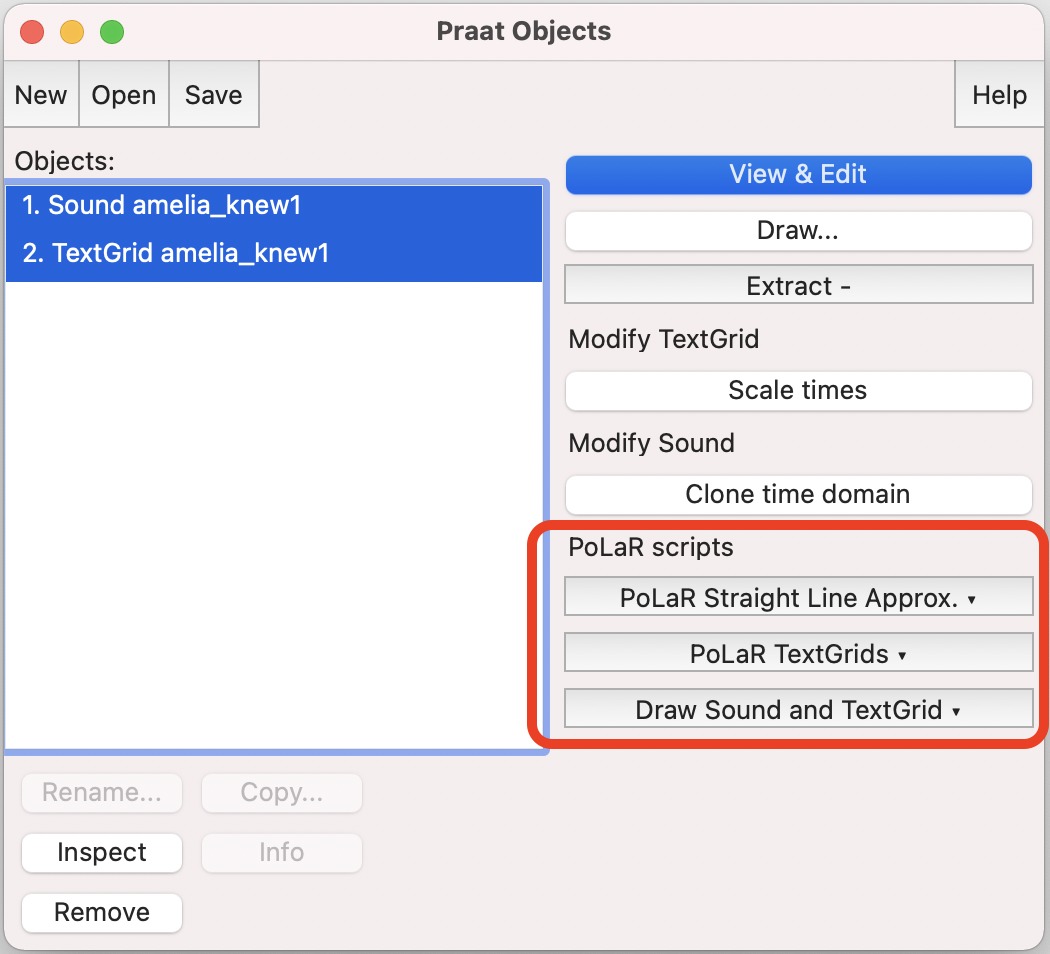
\includegraphics[width=3.75in]{Practical-Plugin-1-Objects-Window-Scripts.png}
		\item Similarly, in an Editor window, the Tier tab menu shows PoLaR plugin commands – it has fewer options but includes links to the most critical scripts\\
			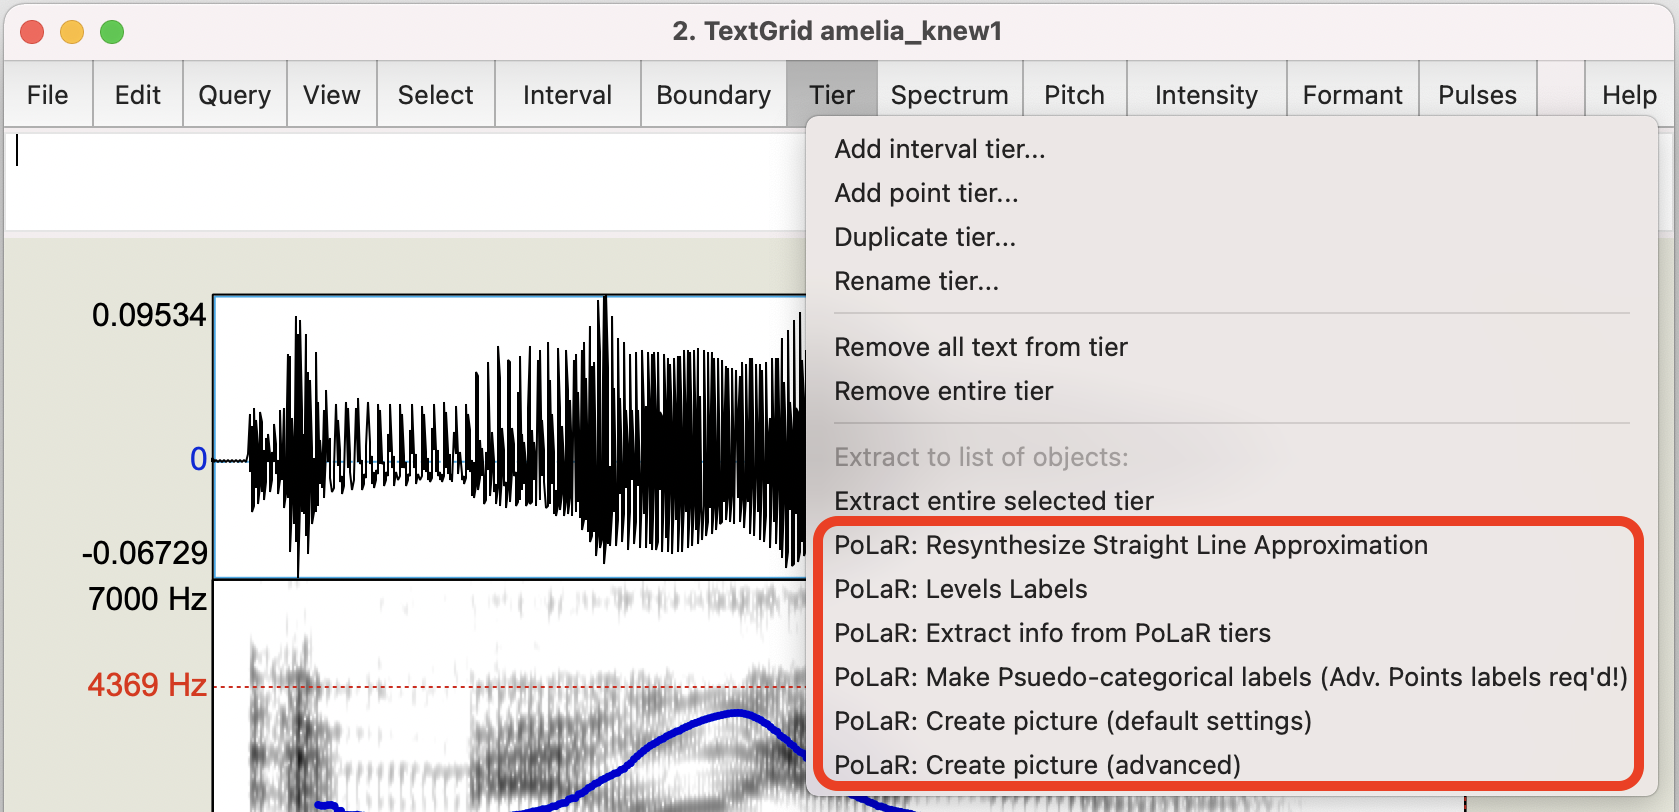
\includegraphics[width=4.5in]{Practical-Plugin-2-Tier-Menu-Scripts.png}
	\end{itemize}
\end{itemize}

\subsection{Functions supported by the PoLaR plugin for Praat}
The PoLaR plugin for Praat enables several functions that may be useful for a PoLaR labeller. The bullet points below name some of these, with other functions (such as the function to resynthesize straight line approximations) being described in section \ref{sec:workflow-with-polar-in-praat} below.

\begin{itemize}
	\item The “Levels Labels” functionality automatically labels the Levels tier
	\begin{itemize}
		\item Once a TextGrid has Points and Ranges annotated, the “Levels Labels” command automatically adds the appropriate values to the Levels tier at the appropriate times (see §\ref{sec:levels}).
		\item Running this script can be done from within an Editor window (for a single Sound\slash TextGrid pair), or from the Objects window on multiple Sound\slash TextGrid pairs.
	\end{itemize}
	\item The “Straight Line Approximations” commands can be used to create an f0 contour based on PoLaR Points labels.
	\begin{itemize}
		\item Once a TextGrid has Points (and ideally Ranges also) tiers labelled, the resynthesize Straight Line Approximation tools can be used to evaluate whether the Points labels capture the essence of the pitch contour (see §\ref{sec:identifying-necessary-points-labels-with-straight-line-approximations}).
		\item When using this tool, be on the lookout for f0-tracking errors and use comma override values to estimate missing or incorrect f0 values (see §\ref{sec:optional-f0-override-labels-for-annotating-pitch-points-without-a-reliable-f0-track}). 
		\item Running this tool can be done from within an Editor window or from the Objects window (when one Sound\slash TextGrid pair is selected).
		\item When this tool is called from the Objects window, the labeller can choose one of three options
		\item[] 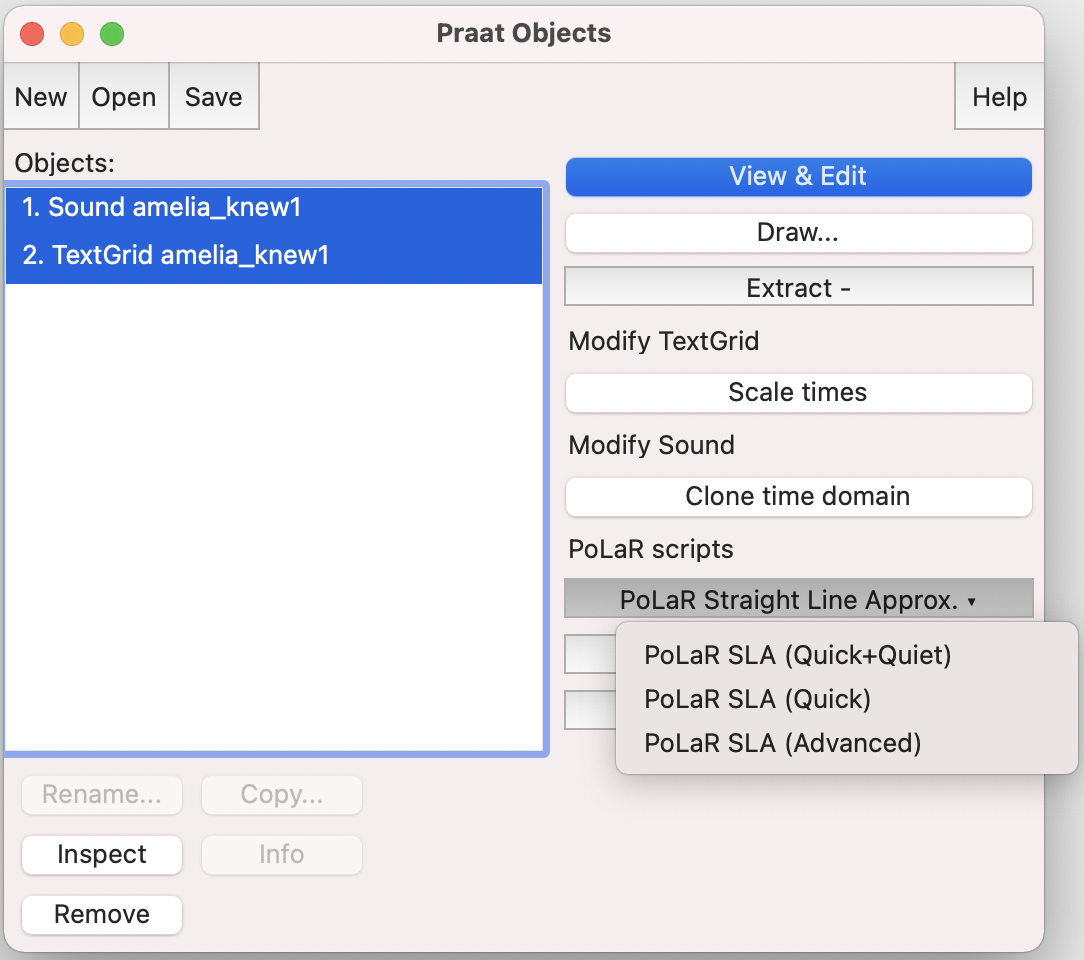
\includegraphics[width=4in]{Practical-Plugin-4-Objects-Window-SLA.png}
		\begin{itemize}
			\item The Quick+Quiet option simply creates the resynthesis, according to default settings.
			\item The Quick option uses default settings as well, and also plays the original and resulting resynthesized versions back-to-back.
			\item The Advanced option gives the user many settings to adjust, and plays the original and resulting resynthesized versions back-to-back.
		\end{itemize}
		\item Note that whenever the tool is used, a resulting Manipulation objects and a new Sound object will appear in the Objects window:
		\item[] 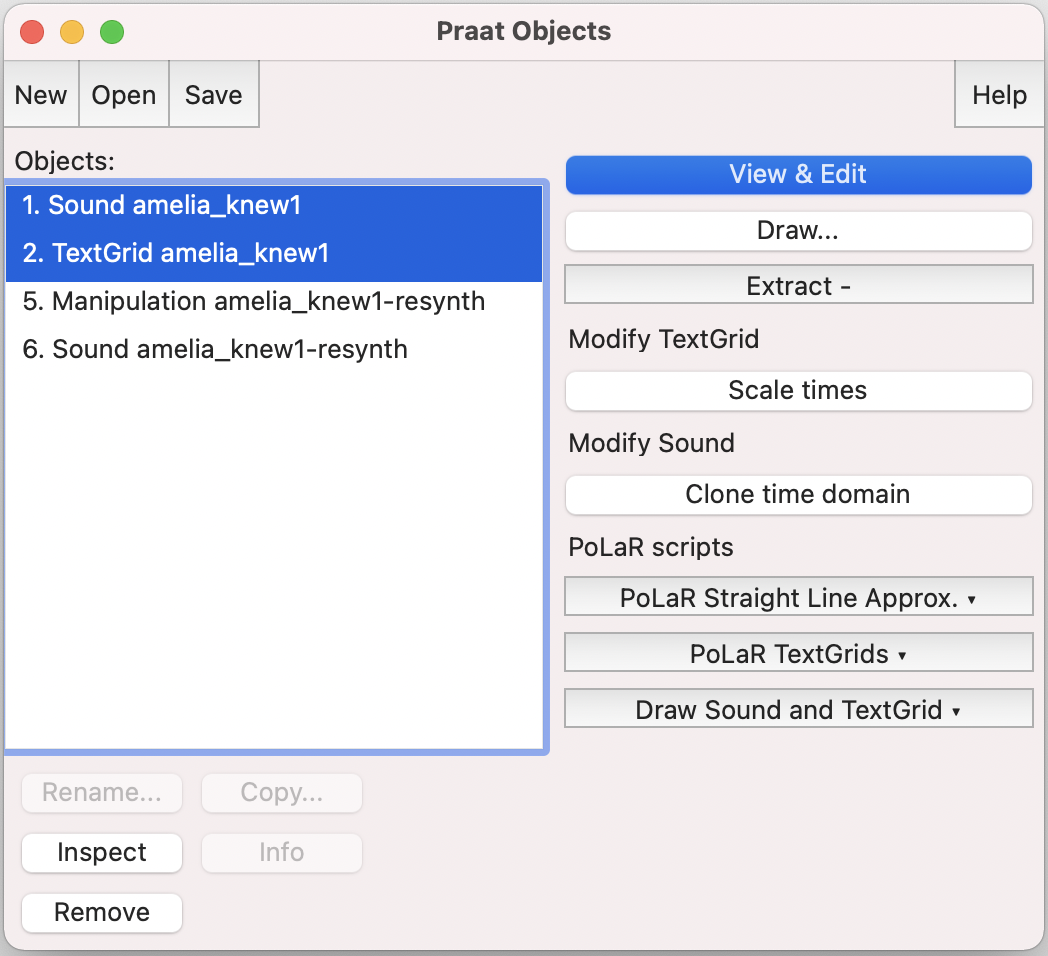
\includegraphics[width=4in]{Practical-Plugin-5-Objects-Window.png}\\
		You can use these files to (re-)play the original and the resynthesized Sound objects and/or to manually adjust the f0 turning points in the Manipulation object.
		\item Labellers are reminded that it is a best practice to iteratively run the SLA resynthesizer while adding\slash removing Points, to ensure that your labels include only and all necessary f0 turning points to felicitously capture the pitch contour.
	\end{itemize}
	\item The “Draw Sound and TextGrid” commands produce figures for publication.
	\begin{itemize}
		\item The default settings are to draw the spectrogram with an overlaid f0 contour above all the tiers of the TextGrid, using the settings described on page \pageref{note on praat settings}.
		\item Running the advanced script opens a new window, where many settings can be manipulated, and other options such as one to allow the user to select which TextGrid tiers to include.
		\item Running this tool can be done from the Objects window or an Editor window.
	\end{itemize}
	\item You can export PoLaR-Related Values to formatted text for spreadsheet software and/or statistical analysis code.
	\begin{itemize}
		\item The information that is exported includes:
			\begin{itemize}
			\item the labels themselves
			\item the timing of the labels (both start and end times, where appropriate)
			\item where the labels occur with respect to intervals on Words and Phones tiers, 
			\item the labels of the Levels and Ranges tiers, where each label occurs
			\item the f0 values at\slash during each label
			\item the intensity values at\slash during the label
			\end{itemize}
		\item Running this tool can be done from the Objects window or an Editor window.
		\begin{itemize}
			\item It can be run on objects loaded into Praat (either from the Objects window or an Editor window): it outputs text that can be copy-pasted into a spreadsheet\footnote{If copy-pasting into an Excel spreadsheet doesn’t separate values across columns, try using “Paste Special” and choose “Unicode Text”.} or into a text file (and then saved as a .tsv [tab separated values] file).
			\item It can be run on all .wav and .TextGrids in a directory (which must have exactly matching file names) by choosing “PoLaR: Extract PoLaR info from files in a directory” from the “New” menu in the Objects window: it outputs data directly into a .tsv file.
			\item Any .tsv file can then be imported into spreadsheet software, fed as input to statistical analysis scripts, or submitted to machine learning algorithms.
		\end{itemize}
	\end{itemize}
	\item You can convert PoLaR labels to pseudo-categorical (AM-style) labels.
	\begin{itemize}
		\item One implementation of an algorithm to do this is in draft state, in the PoLaR plugin for Praat (see §\ref{sec:interspeaker-variation-in-realization-of-prosodic-categories})
		\item Note that, in its current implementation, there needs to be a Phones tier (perhaps previously automatically created by a forced aligner) in addition to Advanced labels on the Points tier
	\end{itemize}
\end{itemize}

There are other planned (i.e., not yet available) functionalities in the PoLaR plugin, which include the ability to automatically estimate (a draft set of) pitch turning points to be used as a starting point for a human labeller creating Points Tier labels. 

\subsection{General Guide to names/functionality of scripts}
Most users of the PoLaR plugin for Praat will not need to explore the .praat files that are the basis of the functionality described here and elsewhere. However, some users may want to delve into these files (e.g., to troubleshoot, better understand the algorithm, or simply run the scripts directly instead of through Praat).

The scripts have been named according to the following conventions:

\begin{itemize}
	\item CORE scripts: contain the core functionality 
	\item DIR scripts: perform the core action on all files in a Directory\slash Folder
	\item SLA scripts: Straight Line Approximation scripts with various options
	\item QUICK scripts: use the default settings (as defined by the QUICK-SETTINGS file).
	\item TGE scripts: Text Grid Editor scripts. Praat makes a distinction between Editor scripts and standalone scripts. All others are standalone. 
	\item TSV scripts: extract information to TSV (tab separated values) files
\end{itemize}


\section{Workflow with PoLaR in Praat}\label{sec:workflow-with-polar-in-praat}

\subsection{Preparing TextGrids}
	\begin{itemize}
		\item Create initial Textgrids with Words and Phones tiers labelled for each Sound file.
		\item Labellers are strongly recommended to use a forced aligner such as the Montreal Forced Aligner (MFA; \citealt{mcauliffe-19}) to do this.
		\begin{itemize}
			\item To use the MFA, first transcribe the speech in XYZ.wav in English orthography, and save that as a (plain text) text file as XYZ.lab (i.e., as a .lab file with a name that matches the .wav file).
			\item Put all pairs of .wav and .lab files for a given speaker into one folder, and run Montreal Forced Aligner (see instructions \href{https://montreal-forced-aligner.readthedocs.io/en/latest/aligning.html}{here}).
			\begin{itemize}
				\item (N.B.: the MFA assumes all paired .wav\slash .lab files that are in the same directory are spoken by the same individual. If there are multiple speakers, place the .wav\slash .lab files into separate subfolders named for each speaker, to get optimal alignments.)
			\end{itemize}
		\end{itemize}
		\item After creating the TextGrid(s) with Words and Phones tiers, open and select all of them in the Praat Objects window.
		\item From the PoLaR TextGrids menu on the right hand side, choose “Blank PoLaR Tiers”
		\item[] 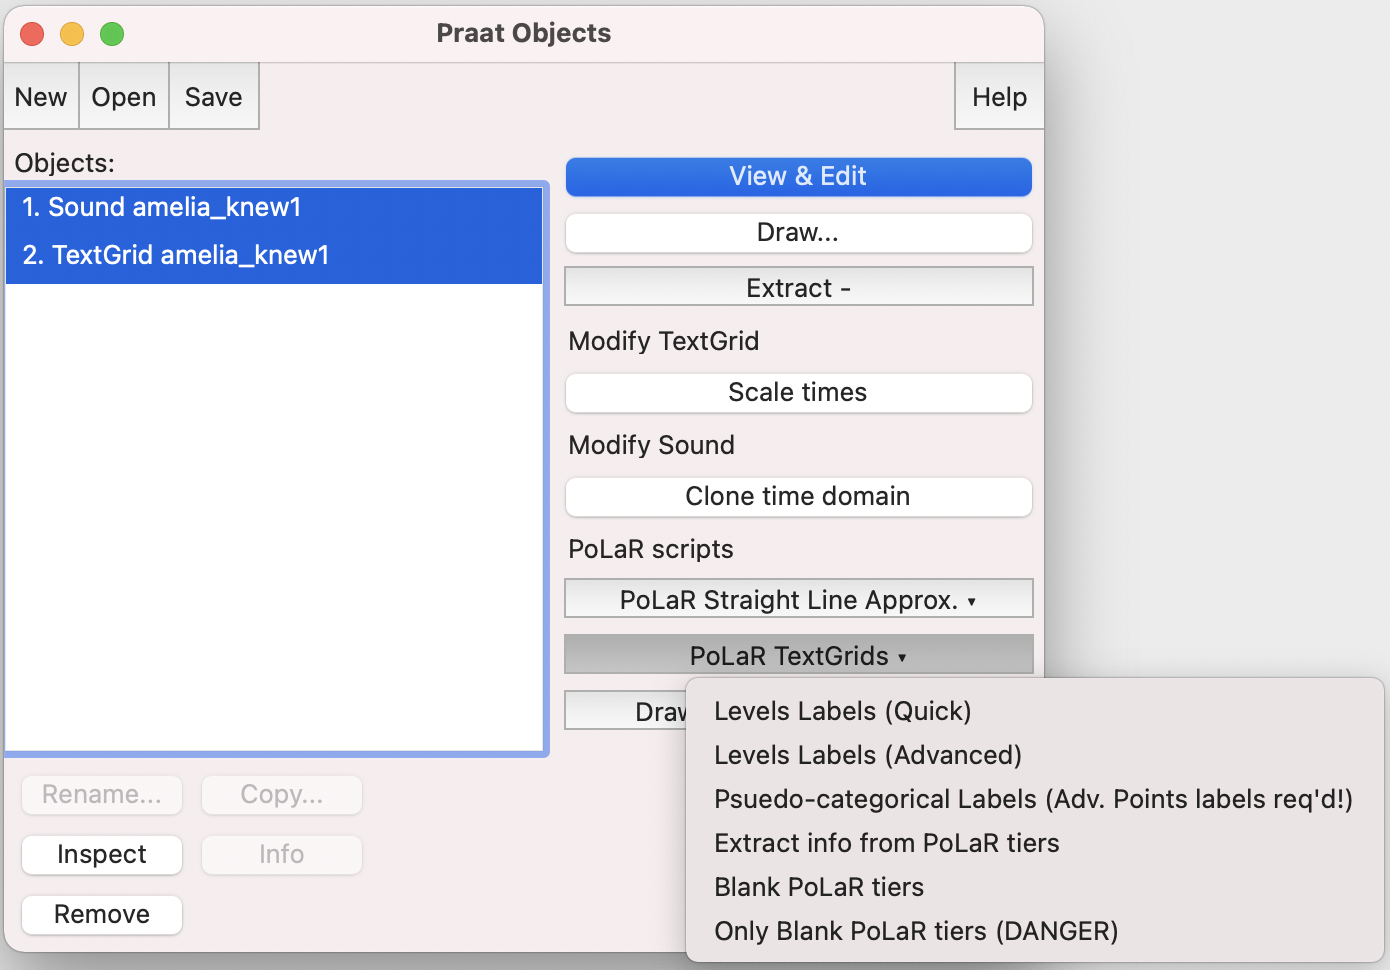
\includegraphics[width=4in]{Practical-Plugin-3-Objects-Window-Textgrids}
		\item This adds the PoLaR tiers to the TextGrid files, leaving them ready to label.
		\item (\textit{Don’t forget to save all TextGrid objects as .TextGrid files!})
	\end{itemize}

\subsection{PoLaR Labelling}	
	\begin{itemize}
		\item Begin PoLaR labelling.
		\begin{itemize}
			\item Most tiers can be labelled in any order (though the Levels tier should be labelled after the Points and Ranges tiers).
			\item Each tier can also be labelled by different individuals, allowing for a “divide and conquer” approach.
			\item It may be easiest to first add Basic PoLaR labels, and then to revise with Advanced PoLaR labels. (It may make sense for the Basic labellers and the Advanced labellers to be different individuals.)
		\end{itemize}
		\item Label the PrStr tier.
		\begin{itemize}
			\item Since this is done according to intuitions of human listeners, there are no automated scripts to use here.
			\item As alluded to in the guidelines, these labels can also be generated on the basis of methodology like those used in RPT tasks (cf. \citealt{cole-14, cole-17}).
		\end{itemize}
		\item Label the Ranges tier.
		\begin{itemize}
			\item Since this is done according to intuitions of human listeners, there are no automated scripts to use here.
			\item As alluded to in the guidelines, Basic labels may attend to the min\slash max attested values, but more Advanced labellers ought to attend to more granular intuitions (cf. §\ref{sec:ranges-advanced}).
		\end{itemize}
		\item Label the Points tier.
		\begin{itemize}
			\item This tier encodes intuitions as well, but there is a tool to help labellers “check their work”:  the Straight Line Approximation resynthesis tool (cf. §\ref{sec:identifying-necessary-points-labels-with-straight-line-approximations}).
			\item Note this tool works best if Ranges tiers are already labelled (but can work without such labels as well).
		\end{itemize}
		\item Label the Levels tier.
		\begin{itemize}
			\item This tier ought to be labelled using the Levels Label tool.
			\item Labellers can use Levels labels to “check their work” with the Ranges tier (e.g., if the pitch at a particular time sounds high to a listener, but has a Levels label of 2 or 3, Ranges labels ought to be revisited; see §\ref{sec:the-influence-of-levels-and-ranges-on-one-another}).
		\end{itemize}
		\item We encourage a practice whereby each file is labelled by multiple labellers, who then discuss labels together after completing their tasks.
		\begin{itemize}
			\item PoLaR labels are specifically designed to facilitate discussions about interlabeller differences; these discussions often result in more fine-tuned labels for a recording, which may provide better analytic results.
		\end{itemize}
	\end{itemize}

\subsection{Post-labelling analysis tools}
	\begin{itemize}
		\item After labelling is complete, there are several analytic approaches one could take; we name a few below.
		\item Impressionistically review the labels.
		\begin{itemize}
			\item Useful for identifying patterns in prominence\slash boundary locations, Levels sequences, Range changes, etc.
		\end{itemize}
		\item Add labels from other labelling systems (e.g., ToBI, IViE, etc.).
		\begin{itemize}
			\item Useful for investigating how categorical labels are realized across utterances / speakers / contexts / etc.
			\item As mentioned in §\ref{sec:interspeaker-variation-in-realization-of-prosodic-categories}, the PoLaR plugin for Praat can create pseudo-categorical labels which may be useful in identifying intonational categories from the bottom-up.
		\end{itemize}
		\item Submit PoLaR labels to statistical analysis\slash computational modelling.
		\begin{itemize}
			\item To do this, the researchers are encouraged to make use of the Extract Info from PoLaR tiers tool, to distill PoLaR labels to various vectors.
			\item (Note this tool can be run on an entire directory of files, through the “PoLaR: Extract PoLaR info from files in a directory” option in the “New” menu of the Praat Objects window.)
		\end{itemize}
	\end{itemize}



\bibliographystyle{glossa.bst}
\bibliography{ch6.bib}

\end{document}	